\section{场论}

\subsection{场的基本概念}

\begin{definition}[等值面]
设 $f$ 是定义在空间区域 $\Omega$ 上的一个数量场.对其值域 $f(\Omega)$ 中的任意一个实数 $c$ ,称点集
\[
f^{-1}(c)=\{M \in \Omega: f(M)=c\}
\]为 $f$ 的一个等值面.
\end{definition}
\begin{figure}[H]
\centering

\includegraphics[width=\textwidth]{场论初步-20250321.png}
% \caption{}
\label{}
\end{figure}

\begin{figure}[H]
\centering
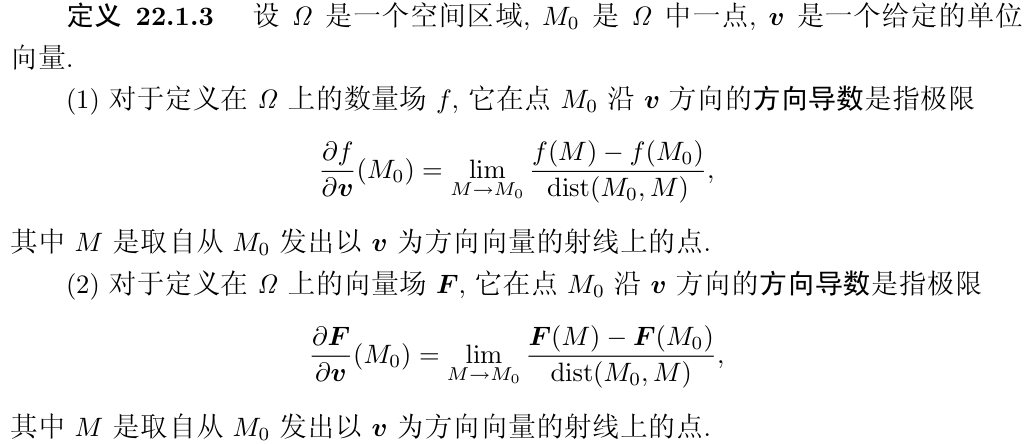
\includegraphics[width=\textwidth]{1-场论初步-20250321.png}
% \caption{}
\label{}
\end{figure}

\begin{figure}[H]
\centering
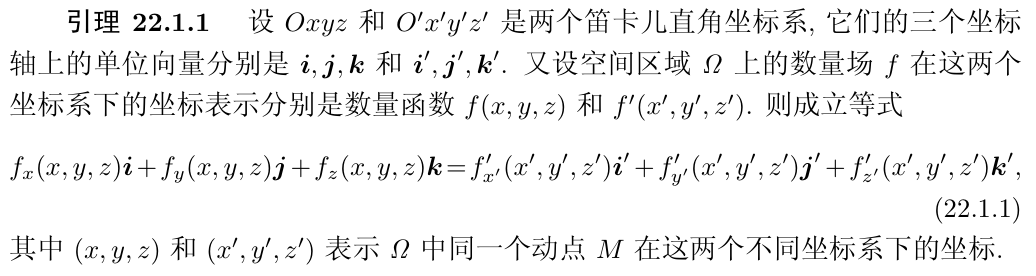
\includegraphics[width=\textwidth]{2-场论初步-20250321.png}
% \caption{}
\label{}
\end{figure}

\begin{proof}
证明考虑使用一大堆正交变换.
\end{proof}

\begin{note}
根据这个引理,如下定义是合理的
\end{note}
\begin{figure}[H]
\centering
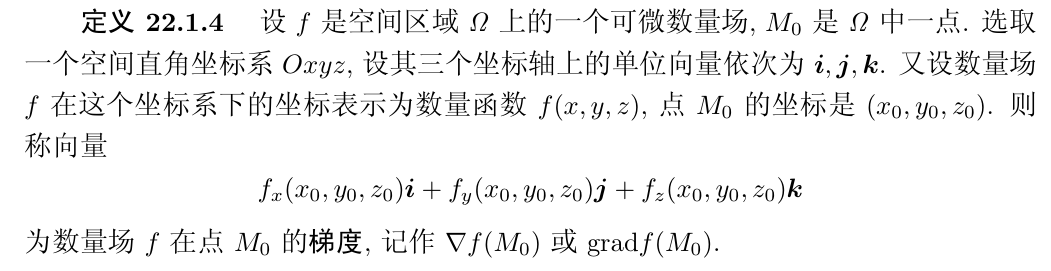
\includegraphics[width=\textwidth]{3-场论初步-20250321.png}
% \caption{}
\label{}
\end{figure}

数量场的梯度有以下性质
\begin{figure}[H]
\centering
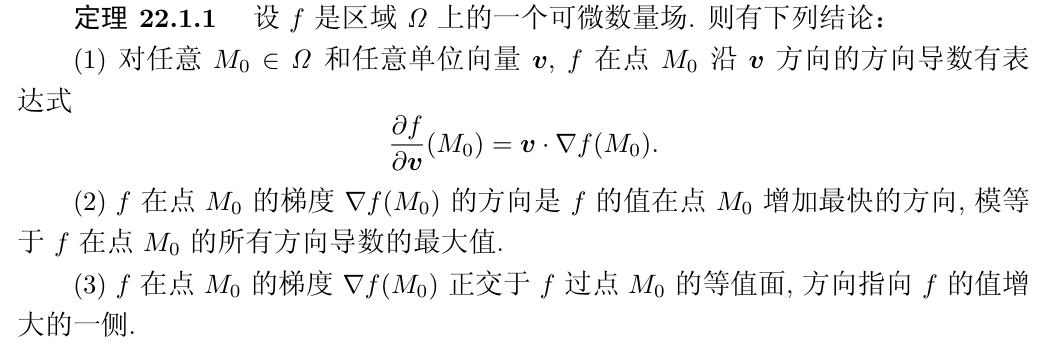
\includegraphics[width=\textwidth]{4-场论初步-20250321.png}
% \caption{}
\label{}
\end{figure}

\begin{figure}[H]
\centering
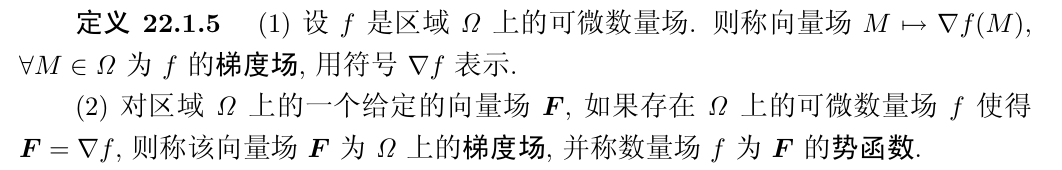
\includegraphics[width=\textwidth]{5-场论初步-20250321.png}
% \caption{}
\label{}
\end{figure}

梯度运算的基本公式如下:

\begin{enumerate}
	\item $\nabla(c)=0(c$ 为常数 $)$ ;
	\item $\nabla(c f)=c \nabla f(c$ 为常数);
	\item $\nabla(f \pm g)=\nabla f \pm \nabla f$ ;
	\item $\nabla(f g)=g \nabla f+f \nabla g$ ;
	\item $\nabla\left(\frac{f}{g}\right)=\frac{1}{g^2}(g \nabla f-f \nabla g)$ ;
	\item $\nabla(f \circ g)=\left(f^{\prime} \circ g\right) \nabla g$ ;
	\item 更一般地,有
\end{enumerate}
\[
\nabla f\left(g_1, g_2, \cdots, g_n\right)=\sum_{i=1}^n f_i\left(g_1, g_2, \cdots, g_n\right) \nabla g_i
\]
其中 $f_i$ 表示函数 $f$ 关于第 $i$ 个变元的偏导数.

\subsection{向量场的通量和散度}

对于封闭区面,本章总规定其单位法向量指向其外侧,即外侧为正侧,内侧为负侧.

\begin{figure}[H]
\centering

\includegraphics[width=\textwidth]{6-场论初步-20250321.png}
% \caption{}
\label{}
\end{figure}

以流体的速度场为例子,当流体速度场穿过 $S$ 的通量大于零时,意味着流体从 $S$ 所包围区域之内穿过 $S$ 流向该区域之外的流量大于从其外部流向区域之内的流量,表明 $S$ 所包围区域内必然有供给流体的源泉. 反之亦然.

因此,向量场 $\boldsymbol{F}$ 穿过封闭曲面 $S$ 的通量反映了 $S$ 所包围区域中产生向量场 $\boldsymbol{F}$ 的物质的正源与负源的某种代数和.

但我们不能了解这种源物质在局部的分布与强弱,因此我们通过\underline{取极限}来达到这样的目的. 给出散度的定义.

\begin{figure}[H]
\centering
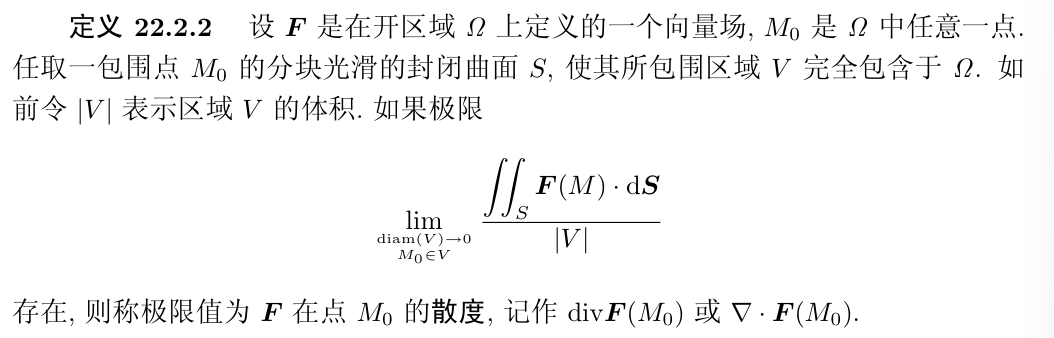
\includegraphics[width=\textwidth]{7-场论初步-20250321.png}
% \caption{}
\label{}
\end{figure}

当向量场 $\boldsymbol{F}$ 在 $M_0$ 的散度 $\mathrm{div}\boldsymbol{F}(M_0)>0$ 时,在 $M_0$ 必有产生向量场 $\boldsymbol{F}$ 的物质的正源,并且 $\mathrm{div}\boldsymbol{F}(M_0)$ 越大这种正源的强度越大,反之亦然.

散度不依赖于坐标系的选取.

\begin{figure}[H]
\centering
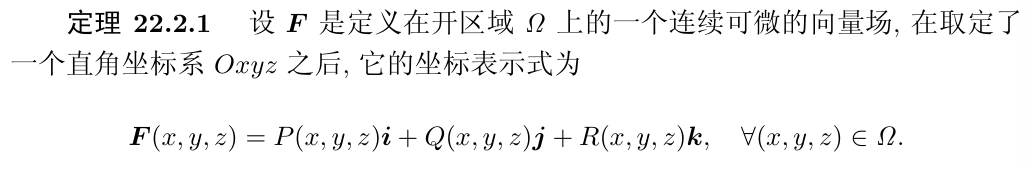
\includegraphics[width=\textwidth]{8-场论初步-20250321.png}
% \caption{}
\label{}
\end{figure}

\begin{figure}[H]
\centering
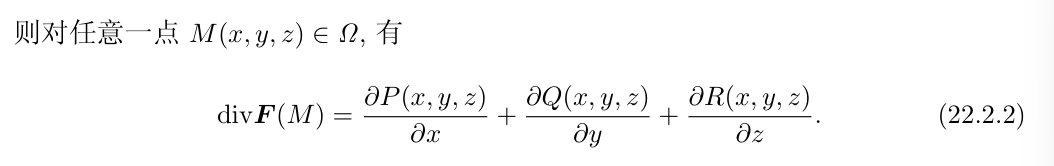
\includegraphics[width=\textwidth]{9-场论初步-20250321.png}
% \caption{}
\label{}
\end{figure}

\begin{figure}[H]
\centering

\includegraphics[width=\textwidth]{10-场论初步-20250321.png}
% \caption{}
\label{}
\end{figure}

散度运算具有以下基本性质:

\begin{enumerate}
	\item $\operatorname{div}(c \boldsymbol{F})=c \operatorname{div} \boldsymbol{F}$($c$ 为常数);
	\item $\operatorname{div}(\boldsymbol{F} \pm \boldsymbol{G})=\operatorname{div} \boldsymbol{F} \pm \operatorname{div} \boldsymbol{G}$ ;
	\item $\operatorname{div}(f \boldsymbol{F})=f \operatorname{div} \boldsymbol{F}+\nabla f \cdot \boldsymbol{F}$ .
\end{enumerate}

\begin{figure}[H]
\centering
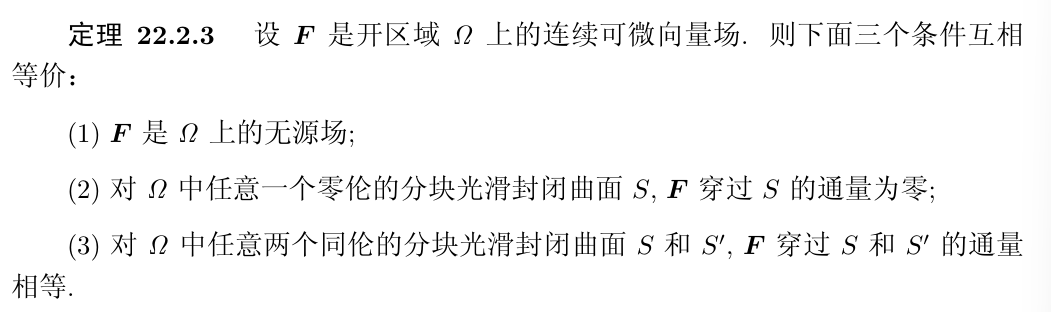
\includegraphics[width=\textwidth]{11-场论初步-20250321.png}
% \caption{}
\label{}
\end{figure}

\subsection{向量场的环量和旋度}

\begin{figure}[H]
\centering

\includegraphics[width=\textwidth]{12-场论初步-20250321.png}
% \caption{}
\label{}
\end{figure}

由公式可以看出,向量场 $\boldsymbol{F}$ 沿封闭曲线 $C$ 的环量反映了 $\boldsymbol{F}$ 沿 $C$ 的旋转情况.

对于流体而言, 速度场沿封闭曲线的环量是否为零反映了曲线是否包围了漩涡的涡管; 当环量非零时, 其正负号反映了曲线的方向是否与它所包围漩涡的旋转方向一致, 其大小则反映了该漩涡的旋转强度.

与散度概念类似,为了了解向量场涡旋的局部分布情况,我们给出方向旋量的概念

\begin{figure}[H]
\centering
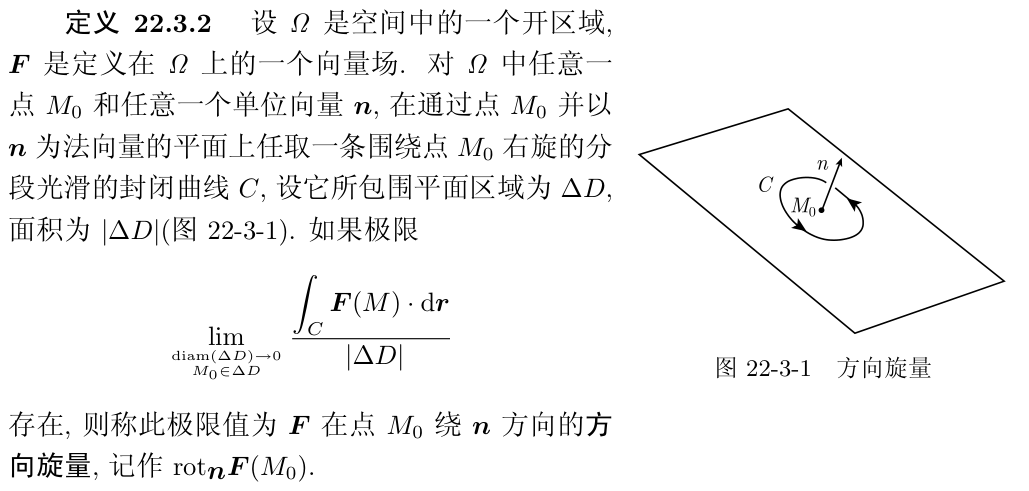
\includegraphics[width=\textwidth]{13-场论初步-20250321.png}
% \caption{}
\label{}
\end{figure}

方向旋量也不依赖于坐标系的选取.

\begin{figure}[H]
\centering
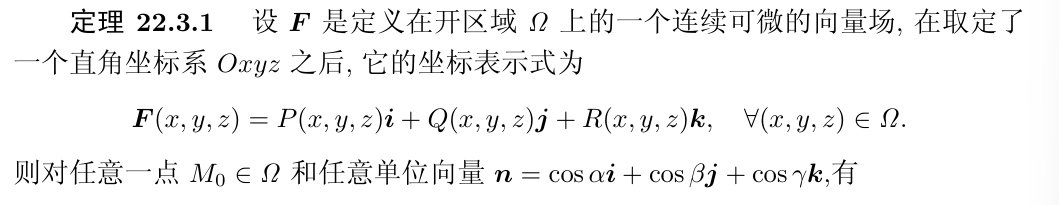
\includegraphics[width=\textwidth]{14-场论初步-20250321.png}
% \caption{}
\label{}
\end{figure}

\begin{figure}[H]
\centering
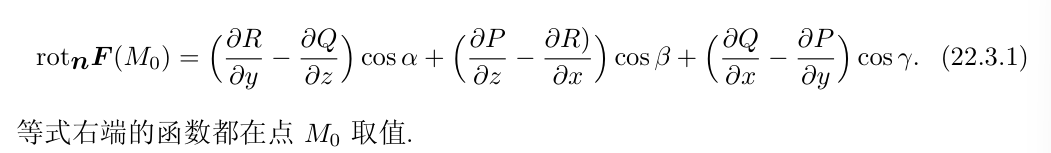
\includegraphics[width=\textwidth]{15-场论初步-20250321.png}
% \caption{}
\label{}
\end{figure}

定义
\begin{equation}
\mathrm{rot}_{\boldsymbol{n}}\boldsymbol{F}(M_0)=\left.\left[ \left( \frac{ \partial R }{ \partial y } -\frac{ \partial Q }{ \partial z }  \right)\boldsymbol{i}+\left( \frac{ \partial P }{ \partial z } -\frac{ \partial R }{ \partial x }  \right)\boldsymbol{j}+\left( \frac{ \partial Q }{ \partial x } -\frac{ \partial P }{ \partial y }  \right)\boldsymbol{k} \right]\right|_{M_0}
\label{8f1ff8}
\end{equation}

则有
\[
\mathrm{rot}_{\boldsymbol{n}}\boldsymbol{F}(M_0)=\mathrm{rot}\boldsymbol{F}(M_0)\cdot \boldsymbol{n}
\]
\begin{definition}[旋度]
由 \cref{8f1ff8} 定义的向量 $\mathrm{rot}\boldsymbol{F}(M_0)$ 为向量场 $\boldsymbol{F}$ 在点 $M_0$ 的\textbf{旋度}.
\end{definition}
旋度也记作 $\nabla \times \boldsymbol{F}$,$\mathrm{curl}\boldsymbol{F}$.

\begin{figure}[H]
\centering
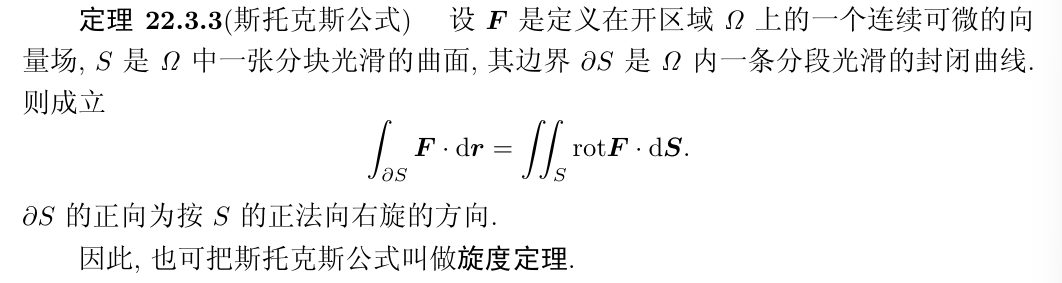
\includegraphics[width=\textwidth]{16-场论初步-20250321.png}
% \caption{}
\label{}
\end{figure}

旋度运算具有以下基本性质:

\begin{enumerate}
	\item $\operatorname{rot}(c \boldsymbol{F})=c \operatorname{rot} \boldsymbol{F}$($c$ 为常数);
	\item $\operatorname{rot}(\boldsymbol{F} \pm \boldsymbol{G})=\operatorname{rot} \boldsymbol{F} \pm \operatorname{rot} \boldsymbol{G}$;
	\item $\operatorname{rot}(f \boldsymbol{F})=f \operatorname{rot} \boldsymbol{F}+\nabla f \times \boldsymbol{F}$ .
\end{enumerate}

引力场和静电场都是无旋场.

\begin{figure}[H]
\centering

\includegraphics[width=\textwidth]{17-场论初步-20250321.png}
% \caption{}
\label{}
\end{figure}

\begin{figure}[H]
\centering
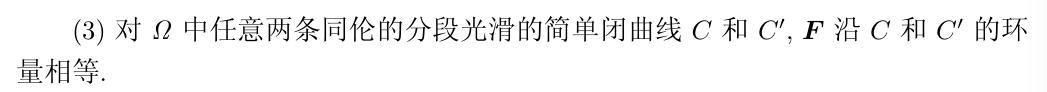
\includegraphics[width=\textwidth]{18-场论初步-20250321.png}
% \caption{}
\label{}
\end{figure}

\subsection{一些重要定理}

\subsubsection{梯度、散度和旋度联合的一些运算公式}

\begin{figure}[H]
\centering
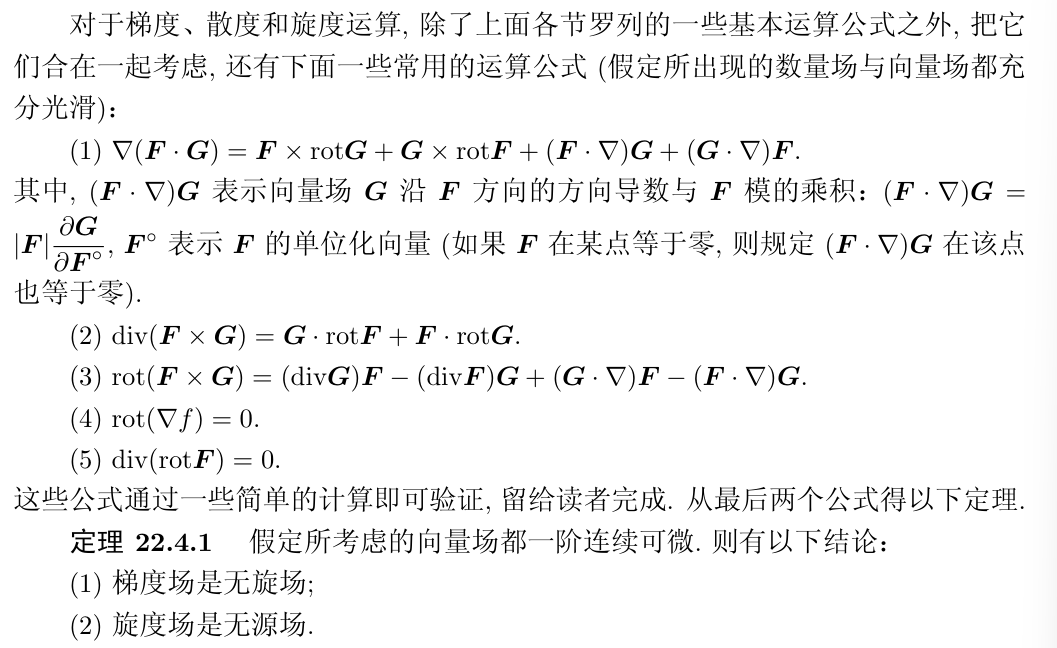
\includegraphics[width=\textwidth]{19-场论初步-20250321.png}
% \caption{}
\label{}
\end{figure}
定义
\[
\Delta=\frac{ \partial^2   }{ \partial x ^2 } +\frac{ \partial^2   }{ \partial y ^2 } +\frac{ \partial^2   }{ \partial z ^2 } 
\]
\begin{figure}[H]
\centering
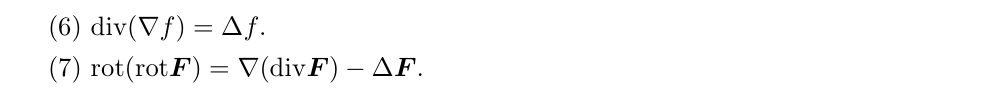
\includegraphics[width=\textwidth]{20-场论初步-20250321.png}
% \caption{}
\label{}
\end{figure}

\subsubsection{保守场及其等价条件}

\begin{figure}[H]
\centering
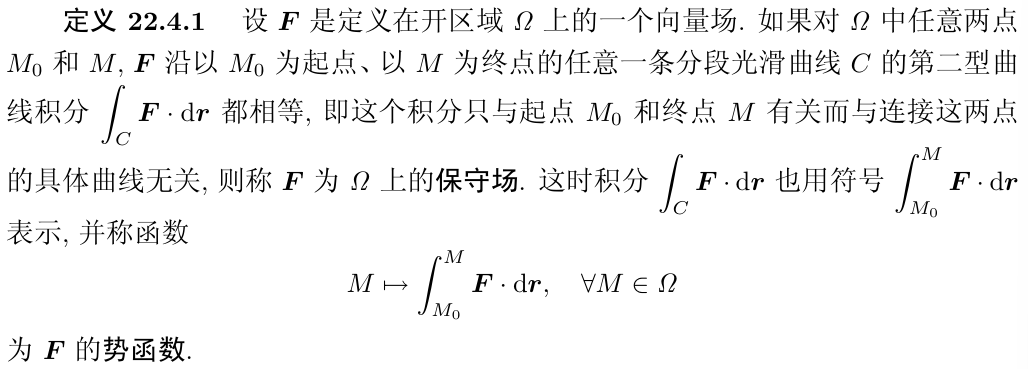
\includegraphics[width=\textwidth]{21-场论初步-20250321.png}
% \caption{}
\label{}
\end{figure}

\begin{figure}[H]
\centering

\includegraphics[width=\textwidth]{22-场论初步-20250321.png}
% \caption{}
\label{}
\end{figure}

\subsubsection{亥姆霍兹分解定理}

下面推导一个重要定理 ——\textbf{亥姆霍兹分解定理}. 粗略地说, 这个定理告诉我们, 每个向量场都可分解为一个无源场和一个无旋场的和.

\begin{figure}[H]
\centering
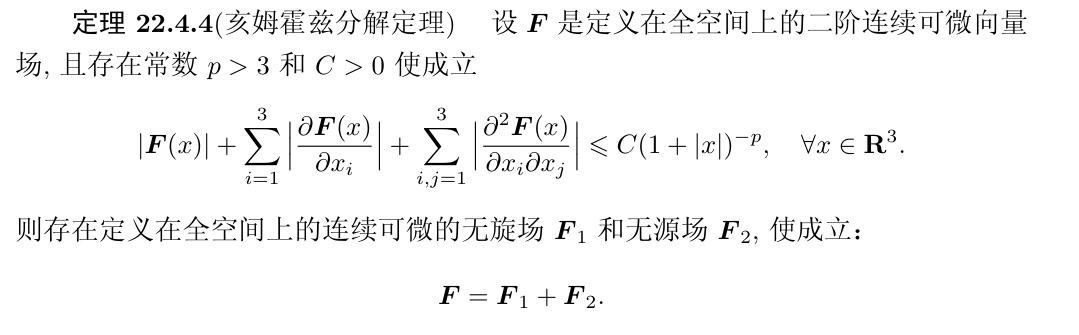
\includegraphics[width=\textwidth]{23-场论初步-20250321.png}
% \caption{}
\label{}
\end{figure}

\begin{figure}[H]
\centering
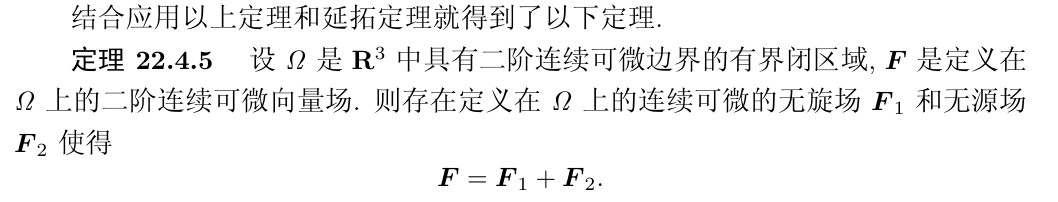
\includegraphics[width=\textwidth]{24-场论初步-20250321.png}
% \caption{}
\label{}
\end{figure}

\begin{figure}[H]
\centering
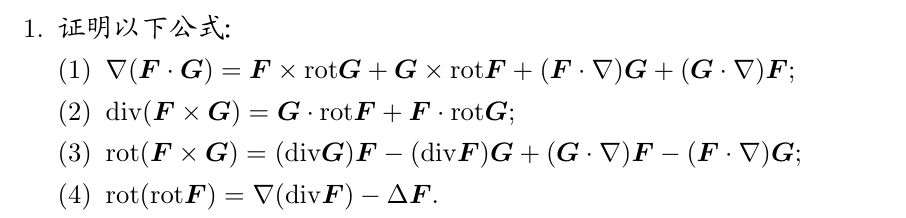
\includegraphics[width=\textwidth]{25-场论初步-20250321.png}
% \caption{}
\label{}
\end{figure}

\subsection{\texorpdfstring{$\mathbb{R}^{3}$}{mathbbR^3} 上}

对于给定的一组标准正交基 $(e_1,e_2,e_3)$,对于标量场 $f=f(x_1,x_2,x_3)$,定义\textbf{梯度}
\[
\nabla f=\frac{ \partial f  }{ \partial x_1 } e_1+\frac{ \partial f  }{ \partial x_2 } e_2+\frac{ \partial f  }{ \partial x_3 } e_3
\]
对于 $\boldsymbol{F}=F_1e_1+F_2e_2+F_3e_3$,定义\textbf{散度}
\[
\mathrm{div}\boldsymbol{F}=\nabla \cdot \boldsymbol{F}=\frac{ \partial F_1 }{ \partial x_1 }+\frac{ \partial F_2 }{ \partial x_2 } +\frac{ \partial F_3 }{ \partial x_3 }
\]
定义\textbf{旋度}
\[
\mathrm{rot}\boldsymbol{F}=\nabla \times \boldsymbol{F}=\mathrm{curl}\boldsymbol{F}=\begin{bmatrix}
e_1 & e_2 & e_3 \\
\frac{ \partial   }{ \partial x_1 }  & \frac{ \partial   }{ \partial x_2 }  & \frac{ \partial   }{ \partial x_3 }  \\
F_1 & F_2 & F_3
\end{bmatrix}
\]
对于 $\boldsymbol{a}=\sum_{i=1}^{3}a_ie_i,\boldsymbol{b}=\sum_{i=1}^{3}b_ie_i$,定义\textbf{叉乘}
\[
\boldsymbol{a}\times \boldsymbol{b}=\begin{bmatrix}
e_1 & e_2 & e_3  \\
a_1 & a_2 & a_3 \\
b_1 & b_2 & b_3
\end{bmatrix}
\]